\documentclass[a4paper]{jpconf}
\usepackage{graphicx}
\bibliographystyle{iopart-num}


\begin{document}
\title{Development of Machine Learning Tools in ROOT}
\author{S. V. Gleyzer$^1$, L. Moneta$^2$, Omar A. Zapata$^3$ }

\address{$^1$ University of Florida}
\address{$^2$ CERN}
\address{$^3$ University of Antioquia and Metropolitan Institute of Technology}
\ead{Sergei.Gleyzer@cern.ch, Lorenzo.Moneta@cern.ch, Omar.Zapata@cern.ch}





\begin{abstract}
ROOT is a framework for large-scale data analysis that provides basic and advanced statistical methods used by the LHC experiments. In particular, these include machine learning algorithms from the ROOT-integrated Toolkit for Multivariate Analysis (TMVA). We present in what follows several recent developments in TMVA. These include a new modular design, new variable importance and cross-validation features, interfaces to other machine-learning software packages and integration of TMVA with Jupyter, making it accessible with a browser.
\end{abstract}


\section{Introduction}
ROOT is an object-oriented data analysis framework that provides statistical methods, visualization and storage libraries for data analysis of high-energy physics (HEP) experiments such as the Large Hadron Collider (LHC) in Geneva, Switzerland \cite{Antcheva20092499}. Although originally designed for HEP applications, ROOT is also widely used in other scientific fields outside of particle physics.\newline\newline 
The ROOT framework provides machine learning tools with the Toolkit for Multivariate Analysis (TMVA) \cite{Hocker:2007ht} including widely-used algorithms in High Energy Physics (HEP) such as:
\begin{itemize}  
\item Fisher and Linear Discriminants (LD)
\item Boosted Decision Trees (BDT)
\item Decision Rule Ensembles
\item k-Nearest Neighbor Classifier (KNN)
\item Shallow Artificial Neural Networks (ANN)
\item Deep Learning Neural Networks (DNN)
\item Support Vector Machines (SVM)
\end{itemize}
Of these, most widely-used methods in HEP are boosted decision trees, neural networks and support vector machines. TMVA provides implementations of these popular methods applicable for machine-learning classification and regression. In the classification context, the machine-learning model is used to separate discrete classes of labeled data, while in the regression context, the machine-learning model is trained to estimate one or more continuous functions, for example the particle energy measured by a HEP detector.TMVA provides a way to compare the performance of these algorithms on the same dataset, allowing for an apples-to-apples comparison useful in choosing the optimal algorithm for a particular analysis task.

\section{New Features and Interfaces}
Recently, TMVA has  been undergoing a significant makeover targeting greater flexibility, modular design and some new features and interfaces. A number of algorithms providing a user with useful information have been added, such as cross-validation and variable importance. Several interfaces to external machine-learning packages have been implemented, and TMVA has been integrated with Jupyter, allowing it to be executed within a browser. In the next sections we describe some of the new functionality and features of TMVA.

\subsubsection{Data Loader}\hspace*{\fill} \\
One of these new design developments in TMVA is the DataLoader class. This class creates greater flexibility and modularity in training different combinations of classifiers and variables. Previously, the choice of variables was defined once and could not be changed later. The DataLoader class allows a packaging of different choices of variables, methods with the data. This design flexibility allows additional functionality, such as cross-validation and variable importance, described in the following sections, to be implemented.\newline\newline
Figures \ref{dl1}, \ref{dl2} and \ref{dl3} show the structure of the DataLoader class. Some of the new features require several Dataloaders at the same time, which is done internally. The same functionality is available to the user as well. Various file formats, for example .root and comma-separated value (.csv) files are supported in DataLoaders.

\begin{figure}[h]
\begin{minipage}{15pc}
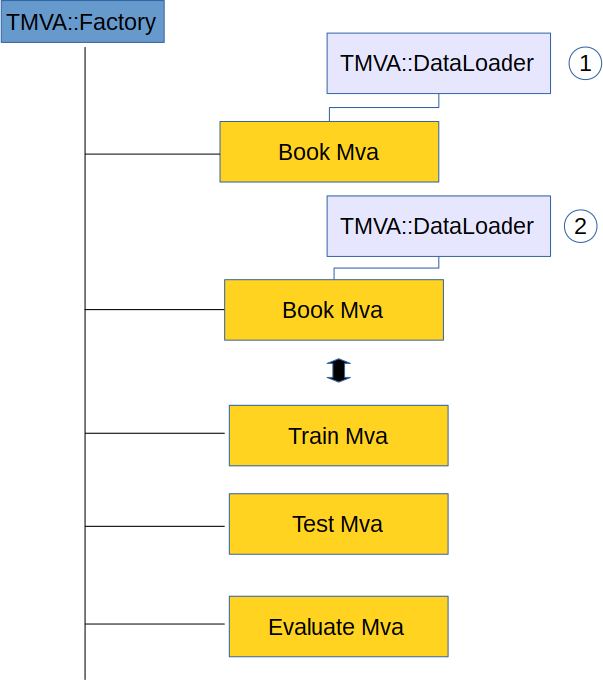
\includegraphics[width=15pc]{img/dl1.png}
\caption{\label{dl1}Booking methods with different dataloaders.}
\end{minipage}\hspace{2pc}%
\begin{minipage}{15pc}
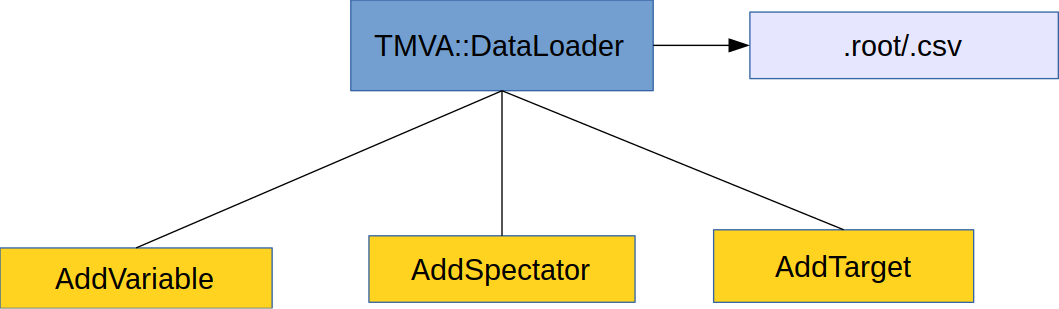
\includegraphics[width=22pc]{img/dl2.png}
\caption{\label{dl2}Loading data from files.}\vspace{4pc}%
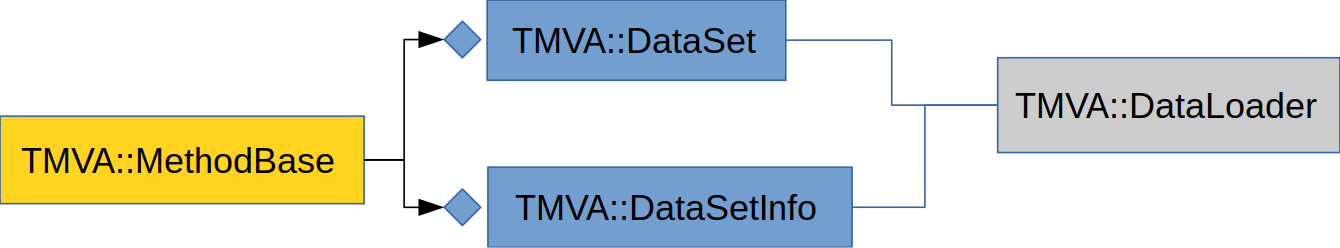
\includegraphics[width=22pc]{img/dl3.png}
\caption{\label{dl3}Storing data in objects in the class MethodBase.}
\end{minipage} 
\end{figure}





\subsubsection{Cross Validation}\hspace*{\fill} \\ 
Cross-validation is a technique for machine-learning model evaluation important for the generalization of the model to unseen data. During k-fold cross-validation, the dataset is partitioned into k folds or partitions. During one cross-validation round, k-1 folds are used for model training, and the remaining fold for model testing. Several rounds of cross-validation are performed with different partitions and model performance results are averaged. One advantage of cross-validation over a simple split into training and testing set, is the ability to use the full dataset to validate the model. Performing cross-validation is known to reduce over-fitting of the data and generally leads to a more accurate estimate of the performance of the machine-learning model on unseen data \cite{arlot2010survey}.\newline\newline 
The first implementation of cross-validation in TMVA consisted of a script calling the TMVA factory, performing dataset splits for different folds and averaging the evaluation results externally. Now, this is done internally in TMVA with a standalone CrossValidation class. Figure \ref{_cv} illustrates five receiver-operating characteristic (ROC) curves for each cross-validation fold showing model performance for each fold for a basic TMVA example. This example has four random variables with gaussian distributions plus several derived variables obtained after applying basic mathematical operations on these variables.

\subsubsection{Variable Importance}\hspace*{\fill} \\
Currently, TMVA provides a number of method-specific variable importance algorithms. Each one is relevant only to the method chosen and is computed during construction. For example, for decision trees variable importance is derived by counting the number of splits for each variable weighted by the square of the information gained from the split,   or for neural networks, as the sum of weights between the inputs and the hidden layer \cite{Hocker:2007ht}.\newline\newline
In addition to these, a new method-independent variable algorithm was added. This algorithm described in\cite{gleyzer2008paradigm} computes variable importance in the context of classifier performance. A number of seeds are randomly generated, each corresponding to a feature subspace. For each seed, individual feature contributions to classifier performance are measured as loss of classifier performance due to the removal of a feature. Figure \ref{_vi} shows a sample variable importance plot for a basic example in TMVA.


\begin{figure}[h]
\begin{minipage}{15pc}
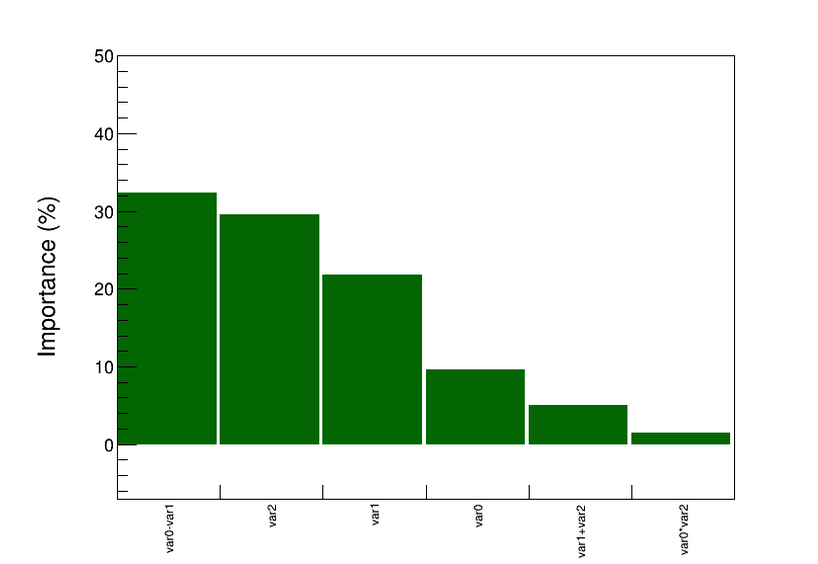
\includegraphics[width=20pc]{img/vi.png}
\caption{\label{_vi} Histogram ranking the variables.}
\end{minipage}\hspace{4pc}%
\begin{minipage}{15pc}
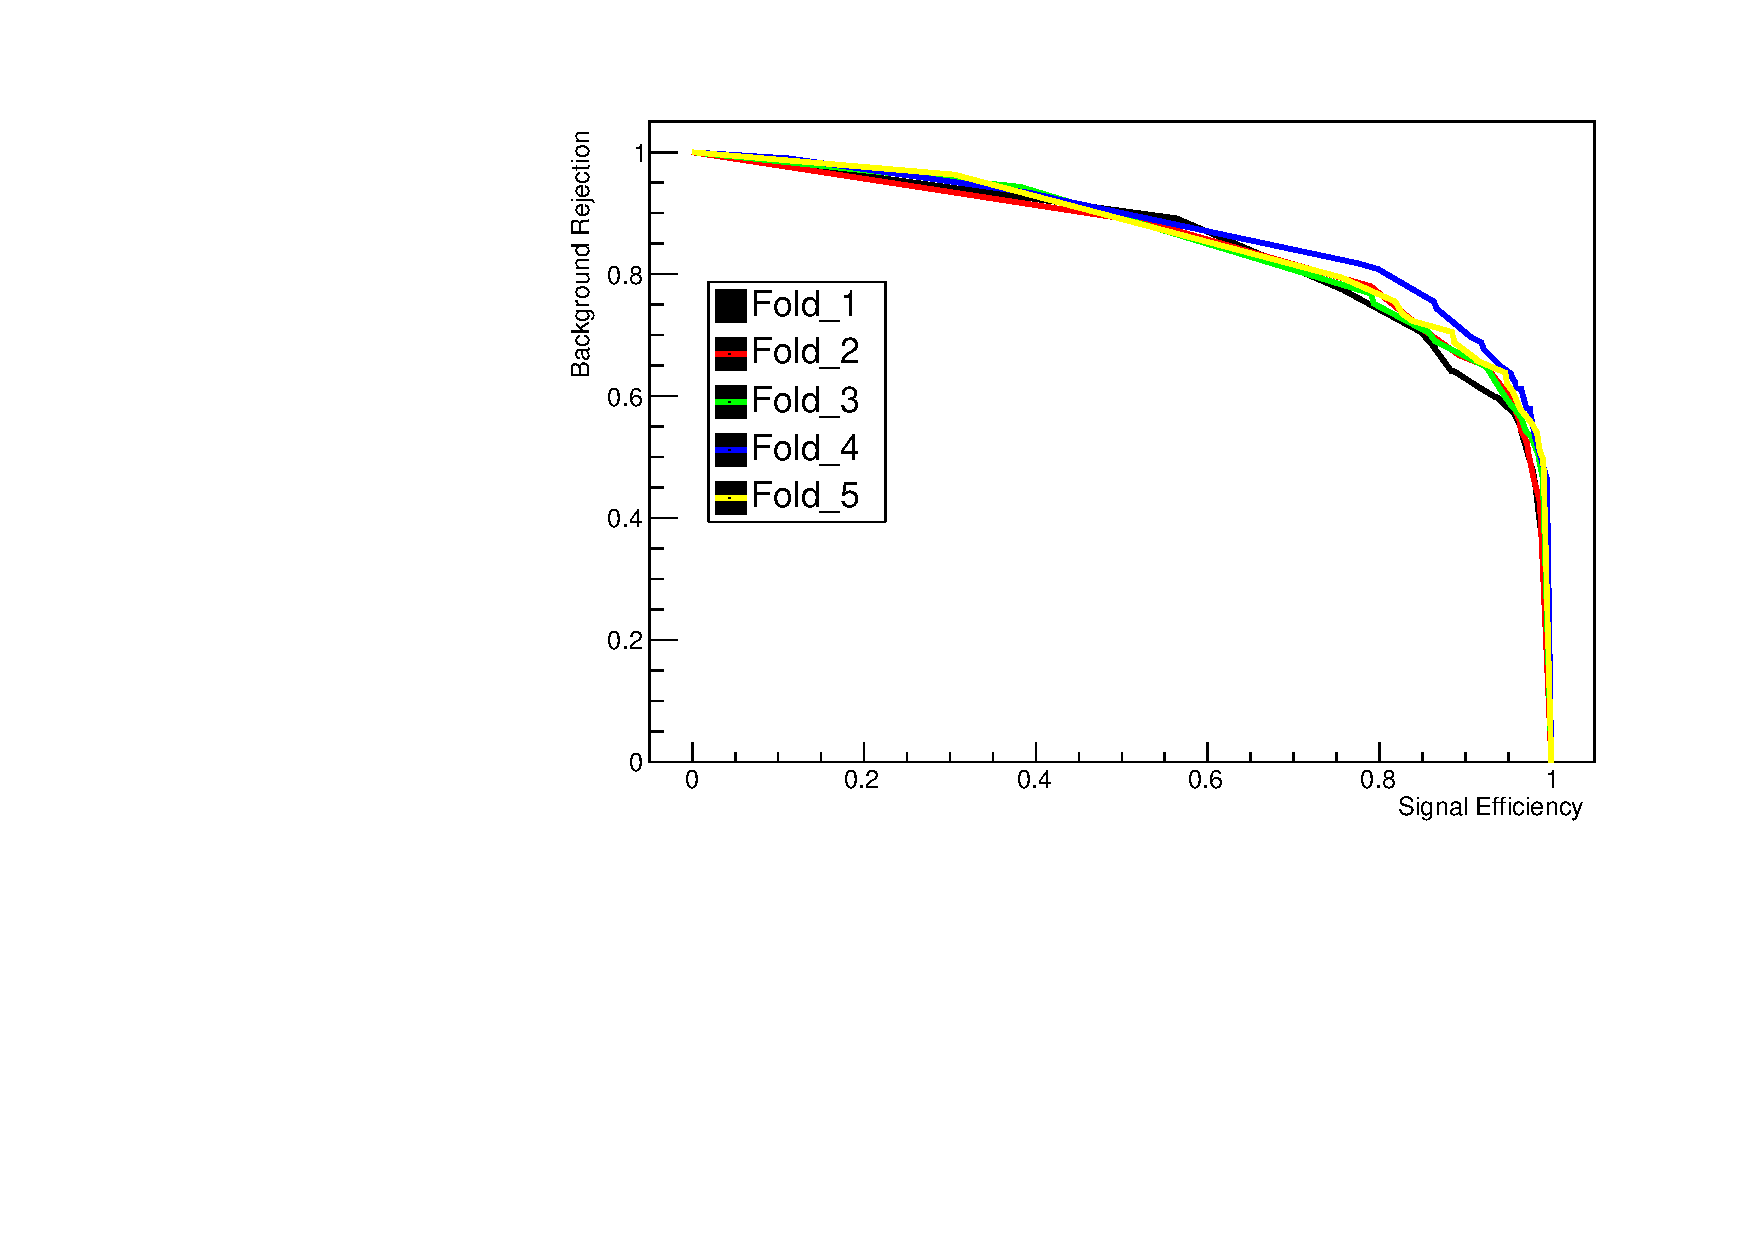
\includegraphics[width=20pc]{img/cv.pdf}
\caption{\label{_cv} Cross validation ROC curves.}
\end{minipage}
\end{figure}

\subsubsection{ROOT-R Interface}\label{ROOTR}\hspace*{\fill} \\
Another useful functionality added to TMVA is the interface to R, called RMVA. R is a free software framework for statistical computing\cite{R}. Prior to the development of RMVA, a ROOT-R interface package was developed that allowed the  use of R functions directly in ROOT. ROOT-R interface also opens a large set of statistical tools available in R, including machine-learning packages, for use within ROOT. Figure \ref{tmva:label} shows the relationship between ROOT, TMVA and other statistical packages like R. The ROOT-R interface design is shown in Figure \ref{rootr:label}. 





\begin{figure}[h]
\centering
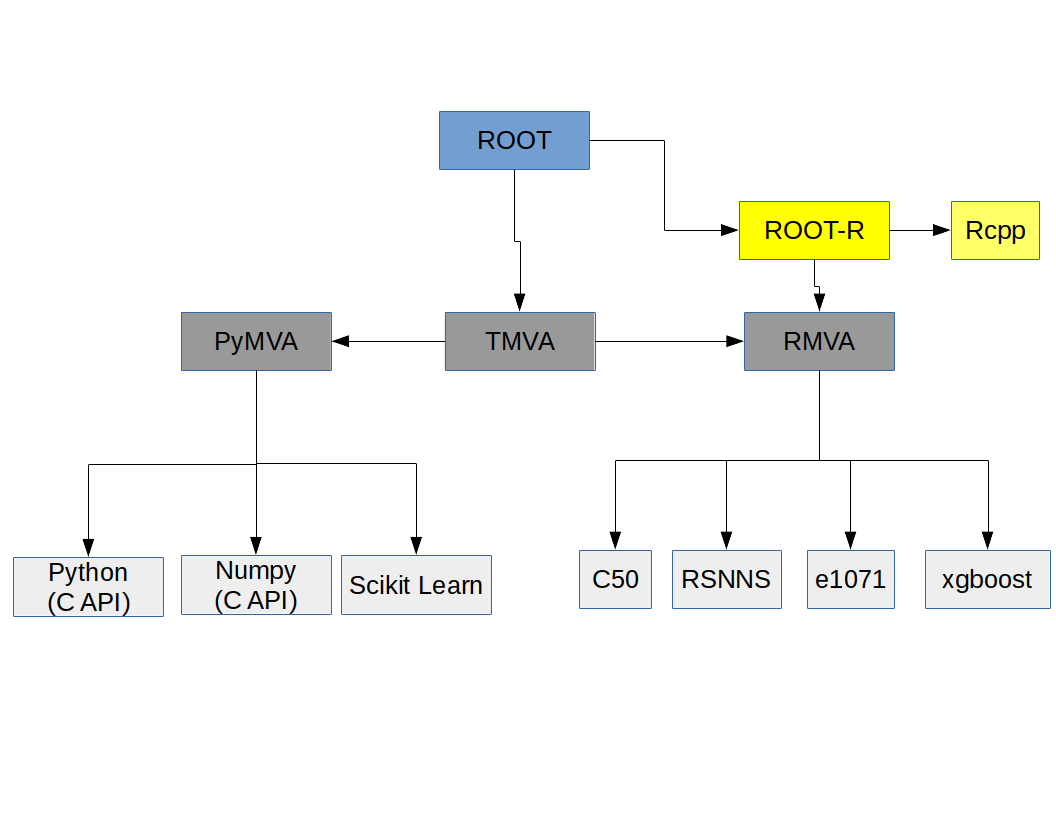
\includegraphics[width=25pc]{img/tmva.png}\caption{\label{tmva:label} Interplay of Machine Learning Tools in ROOT.}
\end{figure}

\begin{figure}[h]
\centering
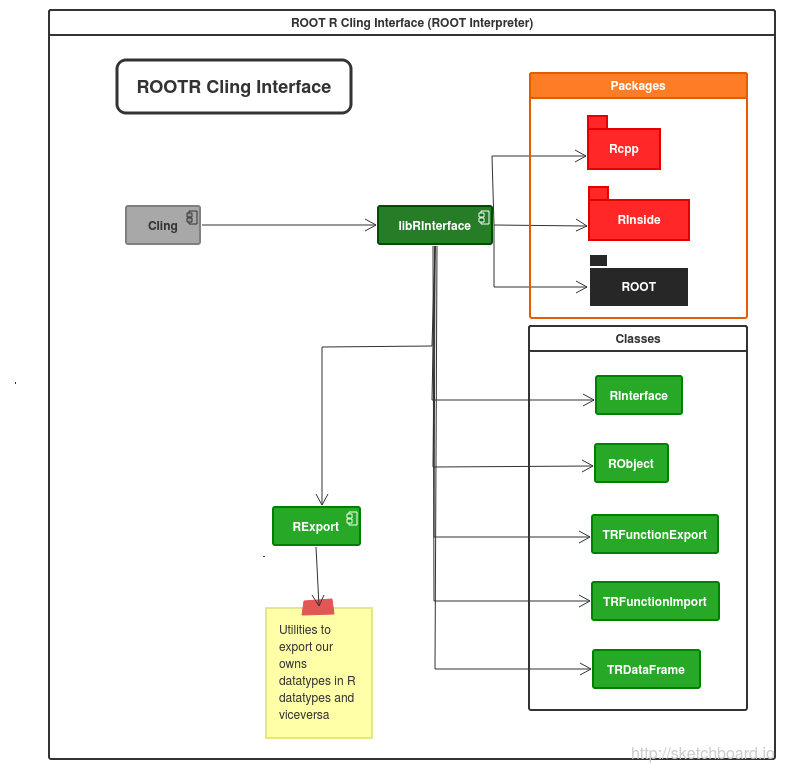
\includegraphics[width=25pc]{img/rootr.png}\caption{\label{rootr:label} ROOT-R Interface design.}
\end{figure}

\subsubsection{RMVA Interface}\label{RMVA}\hspace*{\fill} \\
RMVA is a set of TMVA plugins based on the ROOT-R interface. It allows the use of machine-learning methods available in R directly from TMVA. The goal behind RMVA is not to replace the R package itself but to allow its direct comparison with existing tools in TMVA for a given problem, while adding more methods to TMVA user’s toolbox.\newline\newline
The RMethodBase class in TMVA starts the R environment using ROOT-R, imports the required modules and maps the DataLoader events in R data frame objects using the helper class ROOT::R::TRDataFrame.
Each of the methods inherits from the base class RMethodBase as shown in Figure \ref{rmvaplug}. 
Currently, the following machine-learning packages in R are supported: 
\begin{itemize}  
\item Decision trees and rule-based models (C50) \cite{c50}.
\item Stuttgart Neural Networks in R (SNNS)\cite{rsnns}.
\item Support Vector Machines in R (e1071)\cite{e1071}.
\item eXtreme Gradient Boost (xgboost) An optimized general purpose gradient boosting library\cite{chen2015xgboost}.
\end{itemize}
As shown in Figure \ref{rmvaroc} the above machine-learning methods in R can be executed within the TMVA framework for the basic example.


\begin{figure}[h]
\centering
\begin{minipage}{15pc}
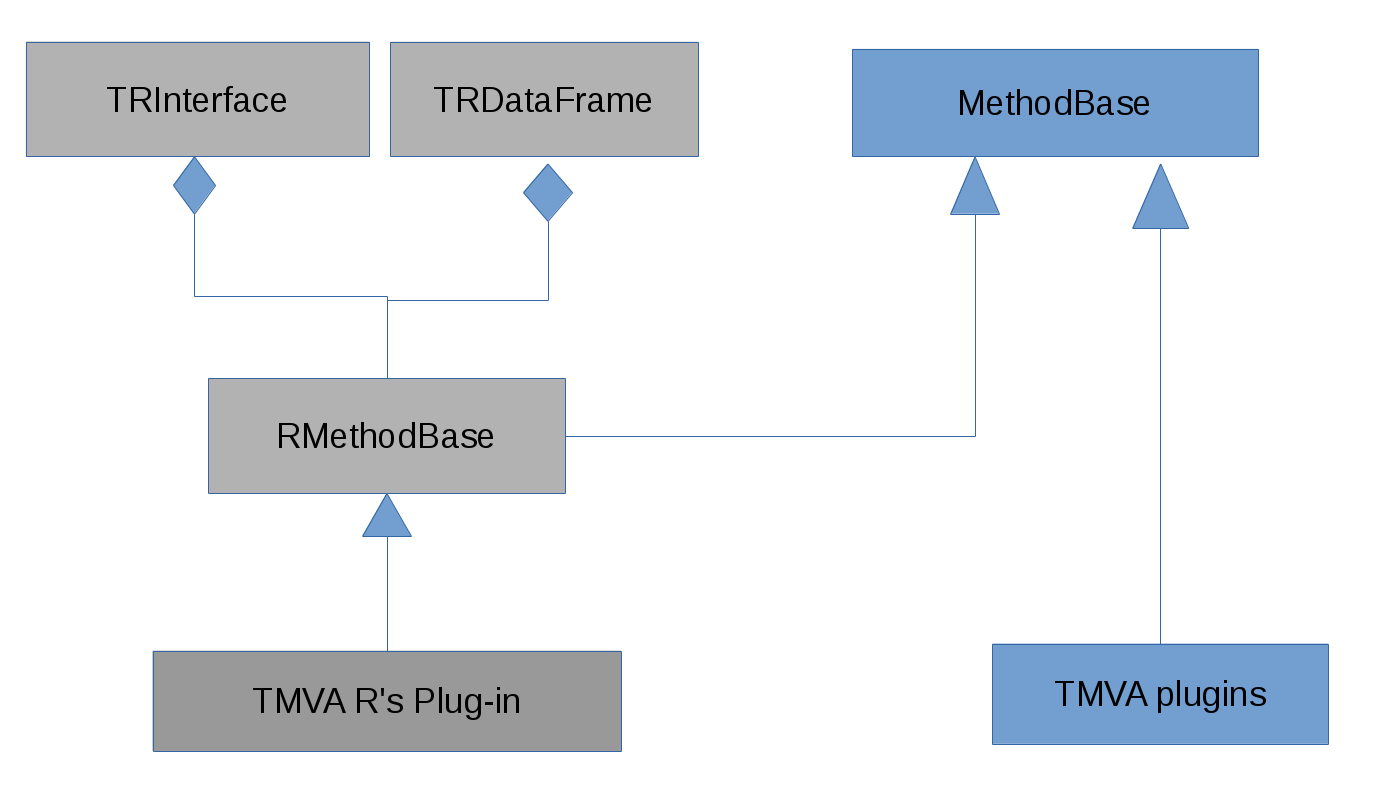
\includegraphics[width=17pc]{img/rmvaplugins.png}
\caption{\label{rmvaplug}RMVA plugins system.}
\end{minipage}\hspace{2pc}%
\begin{minipage}{15pc}
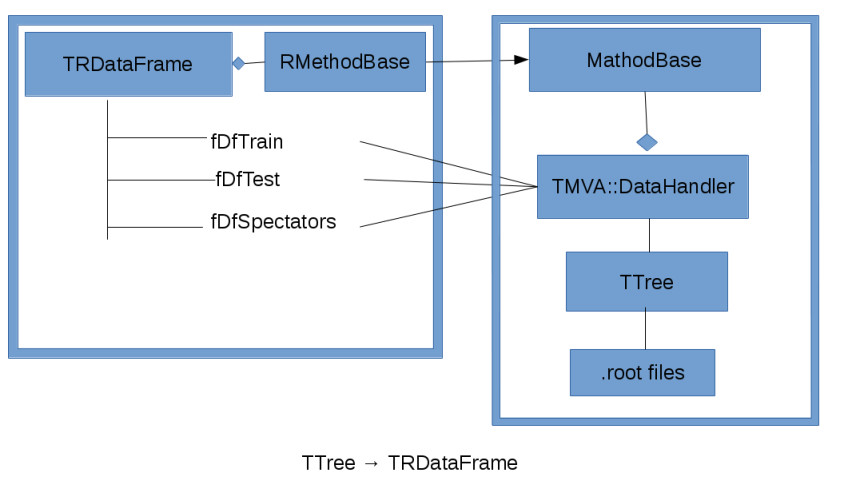
\includegraphics[width=17pc]{img/rmvadf.jpg}
\caption{\label{rmvadf}ROOT-R and TMVA data flow.}
\end{minipage}\hspace{2pc}%
\vspace{2pc}%
\hspace*{\fill} \\
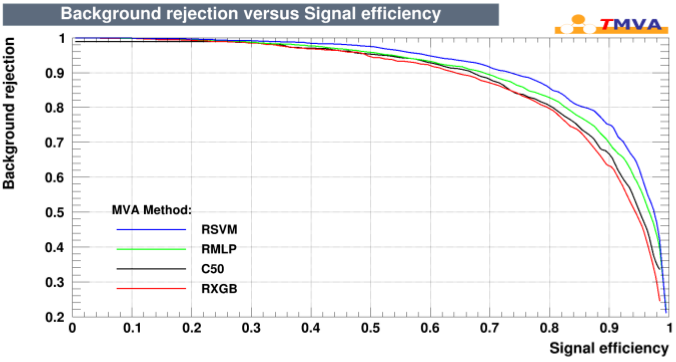
\includegraphics[width=25pc]{img/rmvaroc.png}\caption{\label{rmvaroc} ROC Curves for RMVA methods.}
\end{figure}



\subsubsection{Python with TMVA (PyMVA)} \label{PYMVA}\hspace*{\fill} \\
Similarly to RMVA, PyMVA is a set of TMVA plugins based on Python API that allows direct use of machine-learning methods written in Python from within TMVA. The goal, similarly to RMVA, is not to replace the original method, but to allow the comparison of the method with the other methods in TMVA using the same dataset, selections and performance metrics.\newline
The PyMethodBase class in PyMVA initializes the Python environment, imports the required modules and maps the DataLoader events in numpy arrays using C-API. Each PyMVA method inherits from the base class PyMethodBase, as illustrated in Figure \ref{pymvaplug}. Figure \ref{pymvadf} shows how the dataset is mapped from ROOT trees to numpy arrays. The following python-based methods from \cite{pedregosa2011scikit} are currently available in TMVA which others can be added on demand:
\begin{itemize}
\item Random Forest (PyRandomForest)
\item Gradient Boosted Regression Trees (PyGTB) 
\item Adaptive Boosting (PyAdaBoost) 
\end{itemize}
Figure \ref{pymvaroc} shows the ROC curves of various PyMVA methods for a basic example.


\begin{figure}[h]
\centering
\begin{minipage}{15pc}
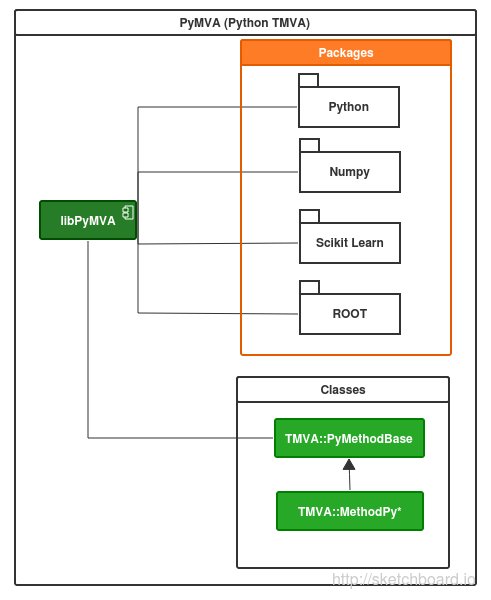
\includegraphics[width=15pc]{img/pymvaplugins.png}
\caption{\label{pymvaplug}PyMVA plugins system.}
\end{minipage}\hspace{2pc}%
\begin{minipage}{15pc}
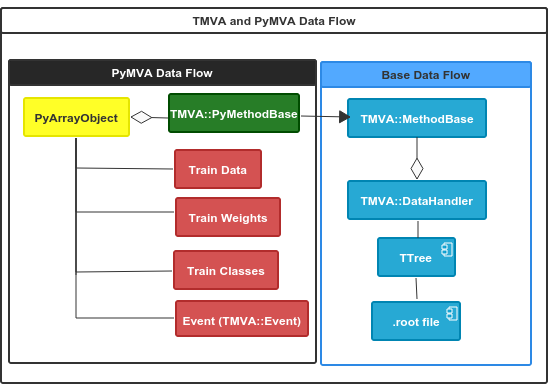
\includegraphics[width=15pc]{img/pymvadf.png}
\vspace{6pc}%
\caption{\label{pymvadf}PyMVA data flow. }
\end{minipage}\hspace{2pc}%
\vspace{2pc}
\hspace*{\fill} \\
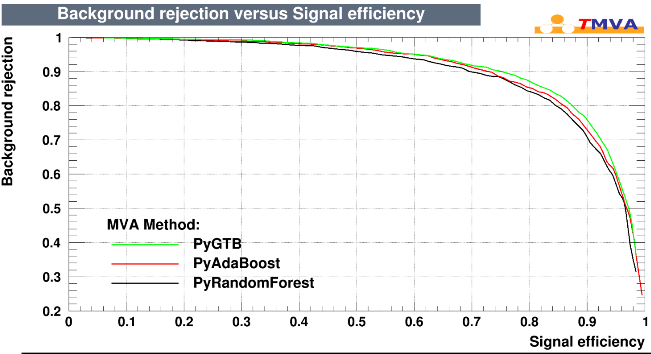
\includegraphics[width=25pc]{img/pymvaroc.png}\caption{\label{pymvaroc} ROC Curves for PyMVA.}
\end{figure}


\subsubsection{TMVA and Jupyter Notebooks}\hspace*{\fill} \\
Another new feature in TMVA is the integration of TMVA and Jupyter Notebooks \cite{PER-GRA:2007}. Jupyter is a web application that combines live code, rich text, links and formulas in a user-friendly format. With the creation of a ROOT Jupyter kernel, additional integration of machine-learning tools in ROOT with Jupyter notebooks became possible. Currently, all the functionality of TMVA is available in Jupyter notebooks, requiring only access to a browser to run and execute TMVA.



\subsection{Conclusions}
Machine learning tools in ROOT have been undergoing a significant makeover and upgrade. In particular, TMVA has a new design targeting greater flexibility and modularity that includes new features such as cross-validation, variable importance and interfaces to R and python-based machine-learning tools. In addition, TMVA is available in Jupyter notebooks, making it accessible through a web browser.



\section*{Acknowledgments}
The work of O. A. Zapata was partially supported by Sostenibilidad-UdeA, UdeA/CODI grant IN361CE and COLCIENCIAS grant 111-556-934918.\newline


\section*{References}

\bibliography{iopart-num}

\end{document}







% \end{document}















































